\section{Architectural Design}\label{sec:arch}

Since the \app solution is based on a modular design, this chapter starts with a description of the whole architecture.
Section \ref{sec:workflow} follows with an explanation of how \app is used in practice.
%Section \ref{sec:comm} details the heart of the solution, NFC communication between Android and NFC terminal and cryptographic measures therein.


\subsection{Building Blocks}\label{sec:arch:det}

%\todo{Vorschlag: Architectural Design nennen und vieles kürzen}

\app's basic architecture consists of the following parts (see figure \ref{fig:arch_ov} for an overview):

\begin{figure}
\centering
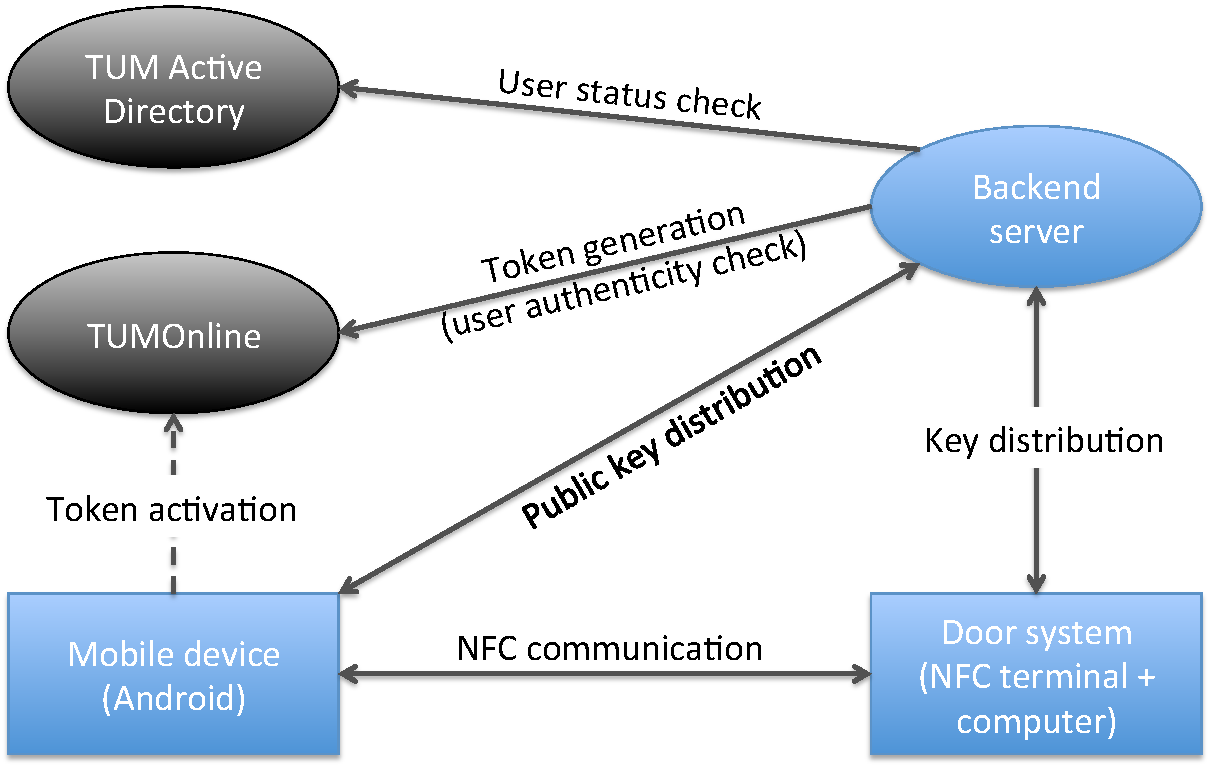
\includegraphics[width=0.8\textwidth]{basic_arch}
\caption{Architectural overview of the \app solution.}
\label{fig:arch_ov}
\end{figure}


\begin{itemize}
\item The smartphone, including a NFC chip as well as an internet connection to register with the service.
An internet connection is only be needed once during initialization of the system or when creating a new key pair in case of revocation.
The smartphone must be able to create an asymmetric key pair and securely store it persistently.
\item The Door Access System, also including a NFC chip which can send and receive.
A simple NFC reader would not suffice as it would be vulnerable to replay attacks.
The door system needs access an intranet in order to check if the student/employee has access to the specific area and to get other information for realizing security features like encryption of the communication.
Therefore, some kind of computer is needed, interacting with the NFC hardware as well as with the backend.
\item A backend system, which checks student ID, the corresponding TUMOnline token and fetches the generated public key from the smartphone.
It finally stores the public key of every registered student.
This local public-key infrastructure is necessary to supply the terminals with an individual public key of each mobile device to deploy a confidential message exchange and a part of authentication.
Furthermore, at every door access attempt it checks the TUM active directory if the person is still a valid student.\\
Important note: All connections to the backend are secured via TLS.
\item The TUMOnline system, which provides a secure way to confirm that a user is real.
This is done via a token that the user has to activate in TUMOnline.
\item The TUM active directory (AD), which has enrolment information about every student and can confirm the status of a person.
\end{itemize} 
The last two items are important for the understanding of the whole solution. They were of course already existing and were not altered for this project.

\bigskip

%Figure \ref{fig:arch_ov} gives a holistic overview of the basic architecture (based on public-key cryptography as discussed in section \ref{sec:alt:proto:pubkey}\todo{brauchen wir die Klammer hier?}):



\subsection{GetInTUM Workflow}\label{sec:workflow}

%\subsection{Registration with Back-end}
\subsubsection*{$\triangleright$ Register a new user}

\paragraph{Step 1)}
To initialize the system, a user (= the user's \app app) has to contact the backend system for authentication.
The user sends his TUM ID and waits for the backend to return a token.
Upon such an user request the backend asks TUMOnline to create a new token.
It then generates a pseudo ID for the user and saves it in a database, together with the corresponding TUM ID and the new token.
This data set is finally returned to the user.
Before proceeding with step 2, the user has to log in to TUMOnline and activate the new token.

\medskip

\noindent This token-mechanism assures the authenticity of a user. Consequences:\\
$\rightarrow$ Only persons with a TUMOnline account can become valid users of \app.\\
$\rightarrow$ A malicious user can generate at most one token for a different person. He cannot flood other users with tokens. Since the `attacked' person will never activate this rogue token, there can be no user account in the backend which does not correspond to a real person.



\paragraph{Step 2)}
After the user has activated his token, his smartphone creates an asymmetric key pair and sends the public part to the backend server.
This key pair will be needed for NFC communications with the door terminal.
Since the door terminal needs to know the public keys of its communication partners, the backend serves as a reliable source to distribute these keys.
Important note: the backend server will reject every attempt to perform this step if the token is not activated by this specific user. The backend can do this check via the TUMOnline Webservice API.



%The back-end system can check if the proposed access token of the user is valid or not via the TUMOnline Webservice API.
%If the user has sent the right access token, the back-end system will demand the public part of the user's asymmetric key pair (which has been created on the user's smartphone before starting the communication).
%In this step, the server will take particular care that the authentic user is in possession of the private part of the transmitted public key and doesn't pretend to be a different identity.



%\subsection{Authentication between Smartphone and NFC Transceiver}
\subsubsection*{$\triangleright$ Authentication between smartphone and NFC terminal}

After the user has registered at the backend system, he can communicate with NFC terminals to open doors. 
A three-way handshake assures a secure connection between smartphone and NFC terminal (see section \ref{sec:comm} for details).
In order to verify the soundness of the procedure, in particular the authenticity of the communication partner, the NFC terminal (i.e.~the system behind it) will fetch the public key of the user who wants to authenticate from the backend system.
Furthermore, the Door Access System will check if the user has access to the requested area (currently, all persons with the status `student' are permitted).
It will finally unlock the door if all checks were positive.

\medskip


\todo{bis hier sollte es jetzt passen}


die anderen zusätzlichen Sachen? Account löschen? Pseudo ID erneuern?\todo{???}
